\documentclass[]{article}
\usepackage{graphicx}
\usepackage{float}


\graphicspath{{./images/}}
\usepackage[spanish]{babel}
\usepackage{url}
\usepackage{booktabs}
\usepackage{natbib}
%opening
\title{Framework Joyeuse}
\author{Jos\'e \'Angel Vald\'ez Torres, Kevin Pe\~na Mora, Yael Atletl Bueno Rojas}


\begin{document}

\maketitle

\begin{abstract}
Framework para crear juegos 3d cuya mec\'anica principal sean los disparos, orientado al rango desde desarrolladores reci\'en iniciados o por iniciarse en el \'ambito, hasta aquellos con conocimiento avanzado. Se compone de una serie de editores entre los cuales se encuentran:
\begin{itemize}
	\item Personajes: Usando una interf\'az simple que permita unificar Inteligencia Artificial, Modelos, animaciones y sonidos. 
	\item Inteligencia Artificial: Mediante un \'arbol de comportamiento.
	\item Niveles: Interf\'az que permita dise\~nar niveles estilo BSP utilizando CSG, evitando as\'i los inconvenientes del alg\'oritmo BSP, pero manteniendo la facilidad de dise\~no que provee. 
	\item Scripts: Mediante un editor ASCII o visual, a elecci\'on del usuario, con la posibilidad de combinar ambos tipos de scripts. 
	
\end{itemize}

\end{abstract}
\newpage
\tableofcontents

\newpage
\part{Entregable 1}
\section{La organizaci\'on}


\subsection{Misi\'on}
Proveer herramientas que faciliten la creaci\'on de v\'ideo juegos, para acercar a personas sin conocimientos de programación al desarrollo de v\'ideo juegos, ya sean artistas, estudiantes, profesores o aficionados. Todo esto, buscando diversificar la industria de los v\'ideo juegos y aumentar el conocimiento de programaci\'on en la sociedad al ofrecer una introducci\'on amena, intuitiva y que acerque al usuario paulatinamente.



\subsection{Visi\'on} 
Ser el est\'andar global para el desarrollo de v\'ideo juegos, solicitado tanto por usuarios novatos como grandes empresas, jugando un papel importante en la construcci\'on del futuro de la industria. 


\subsection{An\'alisis: Fortalezas, Oportunidades, Debilidades, Amenazas}

\subsubsection{Organizacional}
\begin{figure}[H]
	
	\centering
	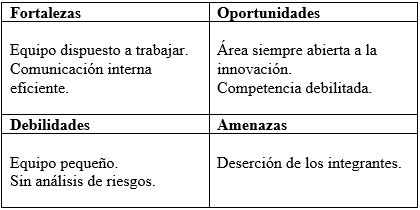
\includegraphics[width=0.6\textwidth]{org}
	\caption{Anal\'isis FODA de la organizaci\'on}
	
\end{figure}


\subsubsection{Jos\'e \'Angle Vald\'ez Torres }
\begin{figure}[H]
	
	\centering
	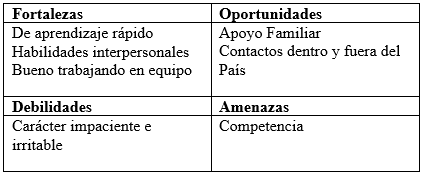
\includegraphics[width=0.6\textwidth]{jose}
	\caption{Anal\'isis FODA: Jos\'e \'Angel}
	
\end{figure}
\subsubsection{Kevin Pe\~na Mora}
\begin{figure}[H]
	
	\centering
	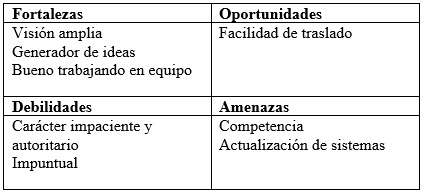
\includegraphics[width=0.6\textwidth]{kevin}
	\caption{Anal\'isis FODA: Kevin}
	
\end{figure}

\subsubsection{Yael Atletl Bueno Rojas}

\begin{figure}[H]
	
	\centering
	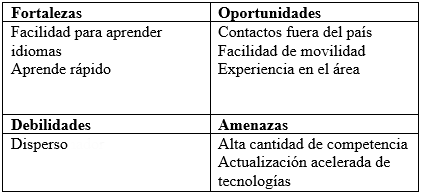
\includegraphics[width=0.6\textwidth]{yael}
	\caption{Anal\'isis FODA: Yael Atletl}
	
\end{figure}

\subsection{Estructura de Desglose de Trabajo}

El trabajo se ha dividido en dos entregables, la documentaci\'on y las herramientas. De parte de la documentaci\'on, se redactar\'an tutoriales y ejemplos, que ser\'an alojados en un sitio web. \newline
En el caso de las herramientas, se dividen en tres componentes b\'asicos, la interfaz para comunicar al usuario con el motor, los prefabricados que conformar\'an la base del juego y las bibliotecas que permiten el funcionamiento de los prefabricados y la interfaz. V\'ease la figura~\ref{EDT}

\begin{figure}[H]
	
	\centering
	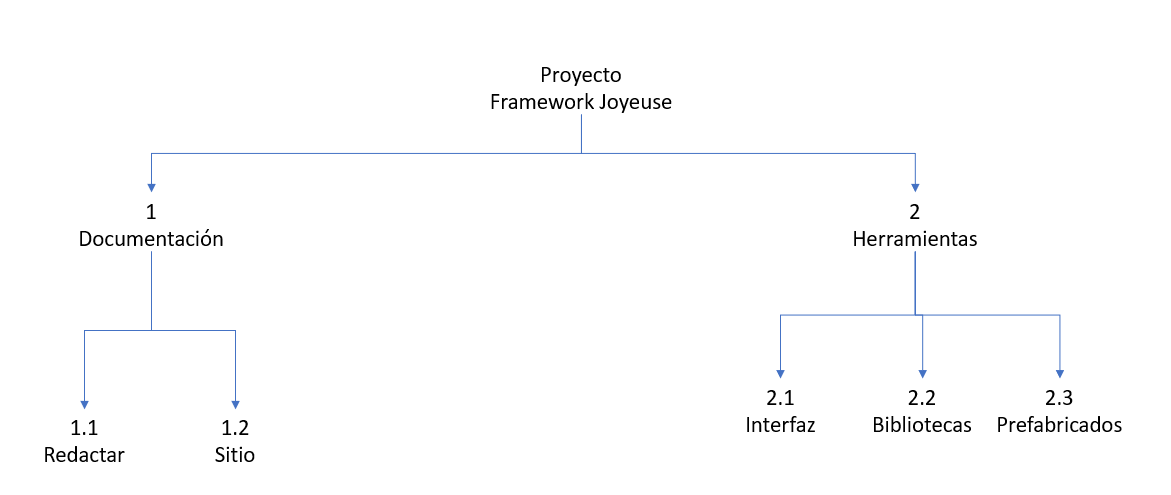
\includegraphics[width=1\textwidth]{EDT}
	\caption{Estructura de desglose de trabajo.} 
	\label{EDT}
	
\end{figure}

%\begin{figure}[H]
%	\centering
%	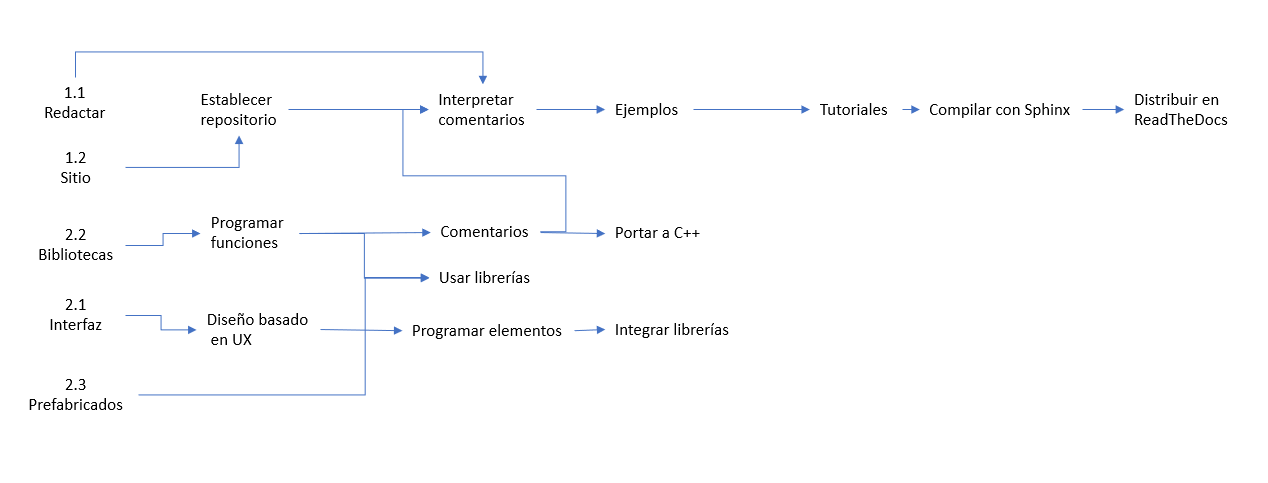
\includegraphics[width=1\textwidth]{EDT2}
%	\caption{Estructura de desglose de trabajo, actividades.}	
%\end{figure}

\section{El Framework}


\subsection{Prop\'osito}

Acelerar el desarrollo 
de videojuegos al permitir a los desarrolladores 
enfocarse en los elementos que vuelven \'unicos a sus
juegos en vez de gastar tiempo en componentes b\'asicos comunes en la industria, adem\'as de facilitar el inicio del desarrollo y aprendizaje para aquellos con nulo conocimiento sobre el tema, ya que le permite crear videojuegos sin temor a encontrarse barreras de c\'odigo a todo aquel que lo desee, acrecentando de esta forma la innovaci\'on creativa en la industria.

\subsection{Importancia}

Al cumplir la doble funci\'on de ser un software R.A.D. (Rapid Application Development) y un Framework, cubre dos campos interrelacionados de la industria que han sido descuidados a trav\'es del tiempo, en cuanto a Shooters respecta. 
Software que funciona con los mismos principios ha quedado obsoleto y olvidado, dejando un hueco que el software existente no podr\'ia llenar debido a su nivel de complejidad.
\newline
Es necesario mencionar el por qu\'e de las decisiones respecto a la orientaci\'on del proyecto: los Shooters acaparar\'an m\'as de 25.9\% del  mercado americano de los v\'ideo juegos para el a\~no 2019, seg\'un la proyecci\'on basada en la figura~\ref{fig:FORB}  y la figura~\ref{fig:STAT} de la p\'agina~\pageref{fig:STAT}.


\begin{figure}[H]
	
	\centering
	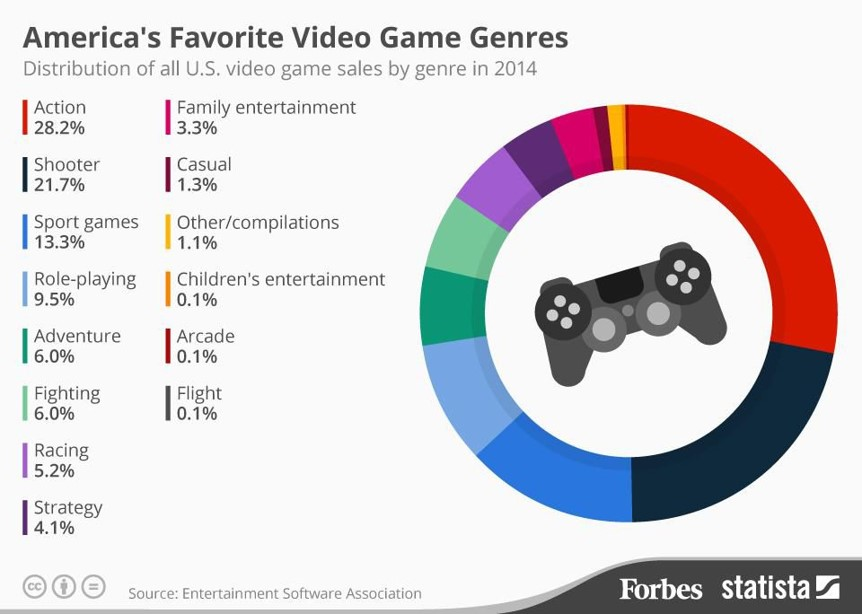
\includegraphics[width=0.5\textwidth]{Picture1}
	\caption{Cuota de mercado, por g\'enero, porcentajes del a\~no 2014.} 
	\label{fig:FORB}
	\cite{Forbes}
	
	
\end{figure}

\begin{figure}[H]
	
	\centering
	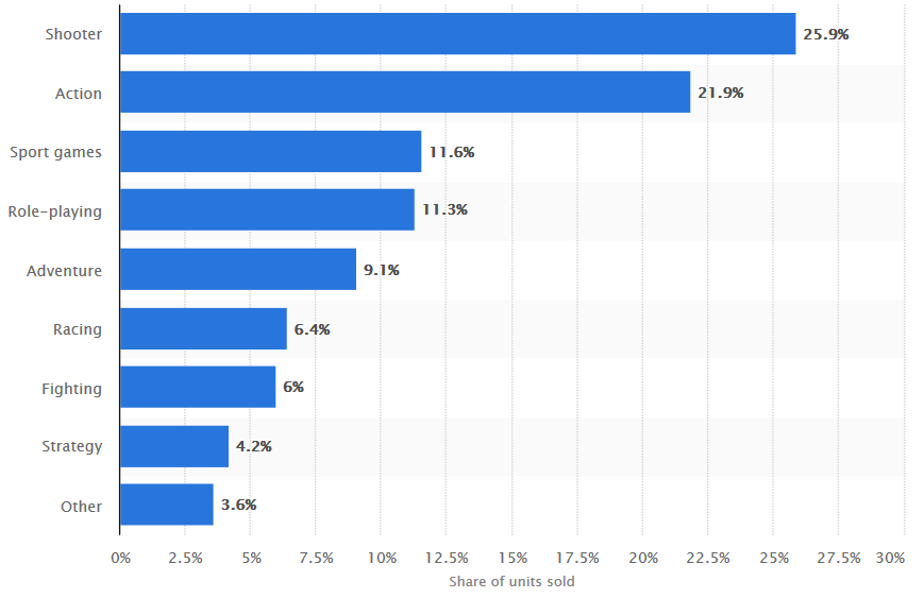
\includegraphics[width=0.5\textwidth]{statista-2}
	\caption{Cuota de mercado, por g\'enero, porcentajes del a\~no 2017.  } 
	\label{fig:STAT}
	\cite{Statista}
	
	
\end{figure}

 Estados Unidos es el segundo mayor cosumidor a nivel global, con ingresos de \$32.7 mil millones de d\'olares, tan solo \$7.5 mil millones debajo de China, tal como puede verse en la figura \ref{NWZOO}.
 El motivo para elegir al mercado am\'ericano sobre al chino, es la libertad de publicaci\'on y contenido que existe en \'este; a diferencia de China, donde los videojuegos est\'an regulados por fuertes restricciones y filtros impuestos por el gobierno. \cite{china1}.
 %Añadir bibliografía

\begin{figure}[H]
	
	\centering
	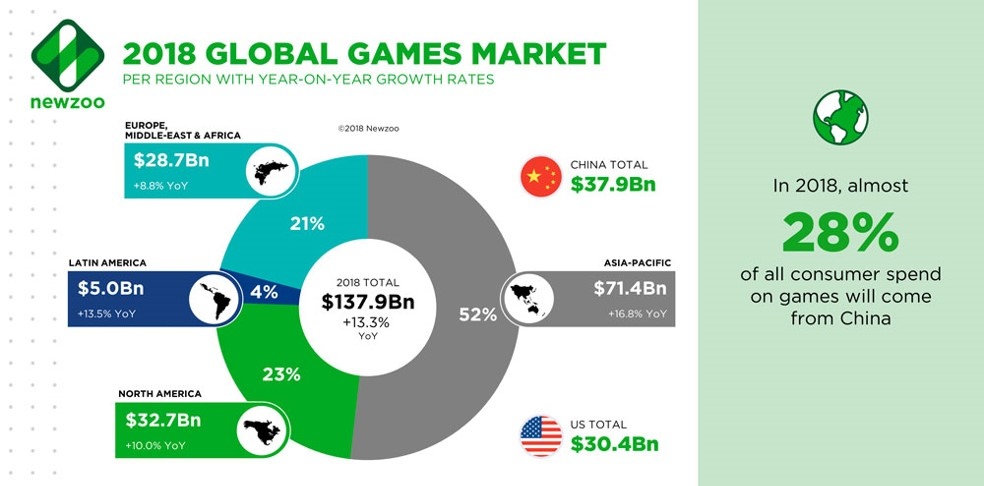
\includegraphics[width=1\textwidth]{GGM2}
	\caption{Procedencia de los ingresos anuales, 2018.  } \cite{Newzoo} 
	\label{NWZOO}
	
\end{figure}

Considerando los puntos anteriores, es posible calcular la proyecci\'on de ingresos para los shooters en el a\~no 2019: considerando las tazas de crecimiento anual, podemos esperar un aumento del 6.45\% en la cuota de mercado, lo que se traduce en 9.54 mil millones de d\'olares en ganancias. 

\subsection{Impacto}
Como impacto secundario al econ\'onmico, para el cual se posee un amplio repertorio de posibilidades, la educaci\'on recibir\'ia un apoyo sustancial, ya que se conseguir\'ia acercar a la programaci\'on a cualquier persona con acceso a una computadora. Por otro lado cabe destacar que se lograr\'ia revivir un sector de la industria cuya oferta decay\'o en a\~nos recientes y que a\'un tiene demanda. Dar una herramienta de este tipo para su uso libre, sin l\'imites para el usuario, ya sean estos de tipo comercial, legal o estructural, permitir\'a el nacimiento de juegos m\'as diversos, ya que se borrar\'a la barrera entre desarrolladores, artistas y jugadores.


\subsection{Trabajo relacionado}

\subsubsection{Entidad 3d}

Creado en el 2004, tuvo un cese del desarrollo entre 2008 a 2013, para ser abandonado finalmente por el creador en 2016. \cite{e3d}. La cantidad de diferentes enemigos, armas, personajes y din\'amicas es limitada. Utiliza niveles BSP (Partici\'on Binaria del Espacio), los cuales limitan el motor a crear juegos en habitaciones y pasillos y exteriores peque\~nos.  
 

Es incompatible con Windows 8 y presenta problemas de compatibilidad con Windows 10, ya que varios paquetes que utilizaba, como DirectPlay, dejaron de ser activados autom\'aticamente desde Windows 7. 



El punto fuerte del motor es su documentaci\'on extensiva, llena de ejemplos pr\'acticos.
Utiliza DirectX8 y OpenGL 1 para renderizar las escenas. \cite{e3d2}.
Su c\'odigo es cerrado, lo que significa que jam\'as volver\'a a recibir una actualizaci\'on. \cite{e3d3}


\subsubsection{GameGuru}

El motor fue creado en el 2012 como sucesor de FPSCreator y a pesar de que el desarrollo est\'a detenido, a\'un recibe mantenimiento y contenido. 
Utiliza LUA como lenguaje de scripts (\#20 en PYPL).
La API gr\'afica que utiliza DirectX11, disponible únicamente en Windows. Otorga la posibilidad de usar modelos y texturas propios, vendi\'endolos tambi\'en como contenido descargable. Se encuentra disponible para ser comprado, bajo c\'odigo cerrado. \cite{game_guru}.

\subsubsection{FPS Creator}

Fue lanzado en 2005, con gr\'aficos DirectX9, su \'ultima actualizaci\'on fue en el 2017 a trav\'es de un mod creado por la comunidad llamado "Black Ice Mod", sin embargo, el multijugador llevaba sin soporte desde el 2015. \cite{MP_discontinued}.

El motor estaba l\'imitado a un uso m\'aximo de RAM de 2GB al momento de la compilaci\'on, lo que se traduce en un m\'aximo de 5 niveles por juego.
S\'olo disponible para Windows.
Actualmente su c\'odigo est\'a alojado en Github, sin una licencia especificada, lo cual deja al motor y posibles modificaciones en ambig\"uedad legal. \cite{FPSCReator}.


\subsubsection{SilentWalk FPS}

Creado en el 2008, recibi\'o s\'olo una actualizaci\'on antes de que parase el desarollo. El nivel de usuarios fue bajo desde siempre e incluso aunque la comunidad sigue existiendo, el sitio oficial dej\'o de tener el enlace a esta desde mayo del 2018. 
Utiliz\'o DirectX 9 en el apartado gr\'afico, su c\'odigo permanece cerrado. \cite{Silentwalk}.

\subsubsection{Reality Factory}

Fue publicado inicialmente en 2006 y recibi\'o su \'ultima actualizaci\'on en el a\~no 2014. Utiliza DirectX9 para los gr\'aficos. La estructura de niveles es BSP y utiliza Simkin como lenguaje de scripts, incluye las herramientas necesarias para crear personajes, objetos, di\'alogos y texturas, tambi\'en incluye modelos, sonidos y texturas para crear prototipos. \cite{features}. Da la opci\'on de cambiar entre c\'amara en primera y tercera persona. De c\'odigo abierto. \cite{overview}.


\subsection{Patentes relacionadas}

\subsubsection{Game production tool supporting multi platform using game development tool}

\paragraph{Resumen}
La presente invenci\'on se refiere a una herramienta de producci\'on de juegos que soporta una plataforma m\'ultiple que usa una herramienta de desarrollo de juegos. De acuerdo con la presente invenci\'on, un art\'iculo, una persona y un fondo que aparecen en un espacio virtual en un juego se definen como objetos del juego y un estado en el que los objetos del juego se muestran en una pantalla en el espacio virtual se genera en forma de M\'ultiples cuadros de imagen se muestran secuencialmente en la pantalla. La presente invenci\'on incluye una unidad de entrada de datos en la que un usuario ingresa datos del juego que incluyen un objeto del juego, dise\~no del juego, planificación del juego y un gui\'on del juego, un módulo personalizado de datos de entrada del usuario que incluye una unidad de conversi\'on de datos que convierte la entrada de datos ingresados en el juego a datos optimizados para la herramienta de desarrollo del juego, un m\'odulo de elementos de la colecci\'on de eventos que genera m\'ultiples listas de eventos que pueden ocurrir durante un juego al analizar los datos optimizados transmitidos desde la unidad de conversi\'on de datos, y un cliente del juego en el que un usuario designa el orden de las m\'ultiples listas de escenas de eventos generadas en el m\'odulo de elementos de la colecci\'on de escenas de eventos para su aplicaci\'on a la herramienta de desarrollo del juego.
\cite{multip}
\paragraph{Comparativa}
Joyeuse, al igual que el programa de la patente, toma informaci\'on a trav\'es de la interacci\'on de un usuario con una interf\'az intuitiva, parecida a un juego, para despu\'es interpretarla para posibilitar que Godot compile el juego. Sin embargo no utiliza un sistema de eventos posibles, se alienta al usuario a crear sus propios eventos a trav\'es del sistema de comandos. 
\subsubsection{Visual game level editing method and system based on trigger}
\paragraph{Resumen}
La invenci\'on describe un m\'etodo y sistema de edici\'on visual a nivel de juego basado en un activador, en el que el m\'etodo comprende los siguientes pasos de 
\newline
\newline A, acceso a una base de datos de desarrollo de juego y actualizaci\'on y obtenci\'on de recursos y datos de dise\~no a nivel de juego; 
\newline
\newline B, que proporciona una interfaz de interacci\'on hombre-computadora, en donde la interfaz de interacci\'on hombre-computadora comprende una regi\'on de edici\'on de estratagema, una regi\'on de edici\'on de nivel y una regi\'on de actividad de configuraci\'on de par\'ametros; 
\newline
\newline
C, carga los recursos de dise\~no a nivel de juego y los datos en elementos en la regi\'on de edici\'on de estratagema y la regi\'on de edici\'on de nivel configurada por un usuario, y traduce al menos un elemento de combinaci\'on de estratagema probado en un archivo de formato de datos de nivel y transmite el archivo de formato de datos de nivel a Una herramienta de edici\'on de nivel de juego para crear o actualizar el nivel. \newline 
\newline El sistema comprende un primer m\'odulo, un segundo m\'odulo y un tercer m\'odulo, en donde el primer m\'odulo se usa para acceder a la base de datos de desarrollo del juego; el segundo m\'odulo se utiliza para proporcionar la interfaz de interacci\'on hombre-computadora; y el tercer m\'odulo se utiliza para exportar el archivo de formato de datos de nivel. El m\'etodo y el sistema tienen las ventajas de que el costo de desarrollo a nivel del juego se reduce obviamente; Se ha mejorado la reutilizaci\'on y la mantenibilidad del c\'odigo.
\cite{leveledit}
\paragraph{Comparativa}

Similar a la forma en la que Joyeuse maneja los ficheros y la interacci\'on proporcionada por el usuario, siendo un paquete comprimido de formato .pck el que cumple la funci\'on de la base de datos. En el caso de Joyeuse, se provee un editor de niveles que se comunica directamente con el motor, guardando la informaci\'on en formato nativo, por lo que no se requiere traducci\'on de datos o formato. 





\subsubsection{Server synchronization graph handle tools}
\paragraph{Resumen} 
La presente invenci\'on se refiere a un m\'etodo para producir contenidos de juegos. Para esto, en la presente invenci\'on, mediante el uso de una herramienta de producci\'on de manejador gr\'afico, se produce un nuevo patr\'on combinando muchos patrones que ya se han producido. Al repetir este proceso, un operador que ha aprendido a usar la herramienta de producci\'on de manejadores gr\'aficos puede revisar y producir f\'acilmente nuevos contenidos sin conocimiento profesional sobre el desarrollo de un juego, y puede extraer el script. Por lo tanto, la presente invenci\'on hace que el mantenimiento sea conveniente.
\cite{Server}
\paragraph{Comparativa}
Tanto el proyecto como esta patente buscan ofrecer la capacidad de producir videojuegos sin tener conocimientos profesionales, sin embargo la patente en cuesti\'on se enfoca a la producci\'on de contenido a trav\'es de patrones y la sincronizaci\'on de los servidores. 














\subsubsection{Tool for video game application development}
\paragraph{Resumen} 
Se describen t\'ecnicas que pueden modificar el contenido de una aplicaci\'on de videojuegos que se ejecuta en una plataforma de juegos. La t\'ecnica incluye el acoplamiento comunicativo con la plataforma del juego para intercambiar mensajes con la plataforma del juego. Una herramienta puede recibir datos representativos de una versi\'on de una pantalla representada por la plataforma del juego. La herramienta puede luego presentar su propia versi\'on de la pantalla y modificar los datos de contenido que conforman la imagen de la pantalla. La herramienta puede enviar un mensaje de modificaci\'on de contenido a la plataforma del juego, el mensaje incluye datos representativos de las modificaciones realizadas por la herramienta. La plataforma del juego puede modificar y generar una nueva versi\'on de la pantalla en la plataforma del juego seg\'un el mensaje de modificaci\'on.
\cite{EA}
\paragraph{Comparativa}
La patente se enfoca en describir un m\'etodo para la comunicaci\'on entre una interf\'az y una plataforma de v\'ideojuegos, para modificar esta misma, enfoc\'andose en la sincronizaci\'on entre la plataforma y el juego en s\'i, no en la creaci\'ona diferencia de Joyeuse que genera y modifica contenido sin depender de una plataforma. 
\subsubsection{Educational game engine capable of directly developing and combining content}
\paragraph{Resumen} 
PROP\'OSITO: se proporciona un motor de juego educativo para implementar f\'acilmente la combinaci\'on de motores y el desarrollo de contenido de un usuario mediante m\'odulos de funciones en una interfaz de programa de aplicaci\'on. 
\newline
\newline
CONSTITUCI\'ON: Un motor de juego educativo incluye una interfaz de programa de aplicaci\'on en un m\'odulo de funci\'on para combinar un motor de juego educativo y un m\'odulo de funci\'on. El motor de juegos educativo es presentado con el lenguaje inform\'atico C ++ que es de f\'acil acceso para un usuario. La interfaz del programa de la aplicaci\'on se configura en base a una tecnolog\'ia orientada a objetos. La interfaz del programa de aplicaci\'on reemplaza un m\'odulo de funci\'on con un m\'odulo de funci\'on de creaci\'on de usuario.
\cite{Edu}
\paragraph{Comparativa}
En este caso, se comparte uno de los objetivos del Framework en el \'ambito educativo, sin embargo en Joyeuse se prefiere utilizar un sistema de comandos interpretados que se asemeje a la escritura de un texto o pseudo-c\'odigo, o en su defecto un sistema de programaci\'on visual a trav\'es de nodos. 

\subsection{Diagrama de Flujo de Datos}

Se tiene un concepto del usuario y el motor Godot como agentes externos, la tarea del Framework es comunicarlos, pasando cifras, modelos, texturas y sonidos que provee el usuario como informaci\'on de compilaci\'on para Godot, empaquetando los ficheros y entregando al usuario un juego distribuible. V\'ease la figura ~\ref{DFD0}. 

\begin{figure}[H]
	
	\centering
	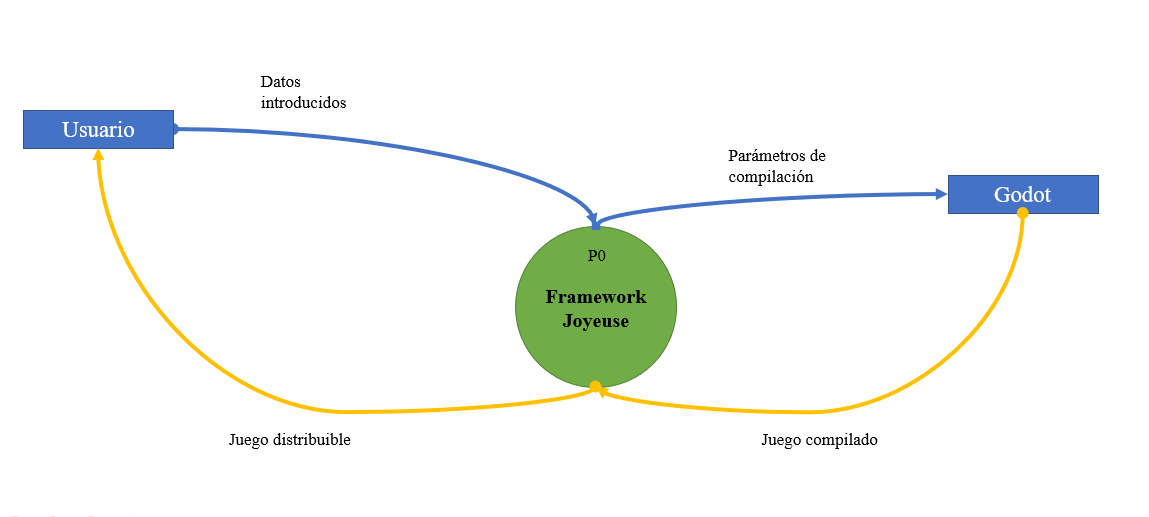
\includegraphics[width=1\textwidth]{DFD}
	\caption{Diagrama de contexto (Nivel 0).} 
	\label{DFD0}
	
\end{figure}

Dentro del Framework, los datos introducidos son clasificados, ya sean estos modelos, sonidos, texturas, archivos de comandos o cifras en bruto. Dependiendo de la clasificaci\'on ser\'an procesados de forma diferente: 
\begin{itemize}
	\item[Comandos] Son interpretados como funciones nativas del motor, que ser\'an usadas para modificar objetos o eventos dentro del juego. 
	\item[Interacci\'on y valores] Son utilizados para crear y modificar los prefabricados y escenas del juego. 
	\item[Sonidos, texturas y modelos] Son ordenados dentro de un directorio con varios subdirectorios y despu\'es almacenados en un fichero comprimido de formato PKG, respetando el orden de los directorios
\end{itemize}
Una vez procesada la informaci\'on de entrada, el Framework mandar\'a las instrucciones de compilaci\'on a Godot, el cual devolver\'a el juego compilado. 
Dentro del Framework, se toma el programa y se adjunta al fichero PKG, d\'ando ambos al usuario para que pueda distribuir su juego. Para un ejemplo gr\'afico, v\'ease la figura~\ref{DFD1}.

\begin{figure}[H]
	
	\centering
	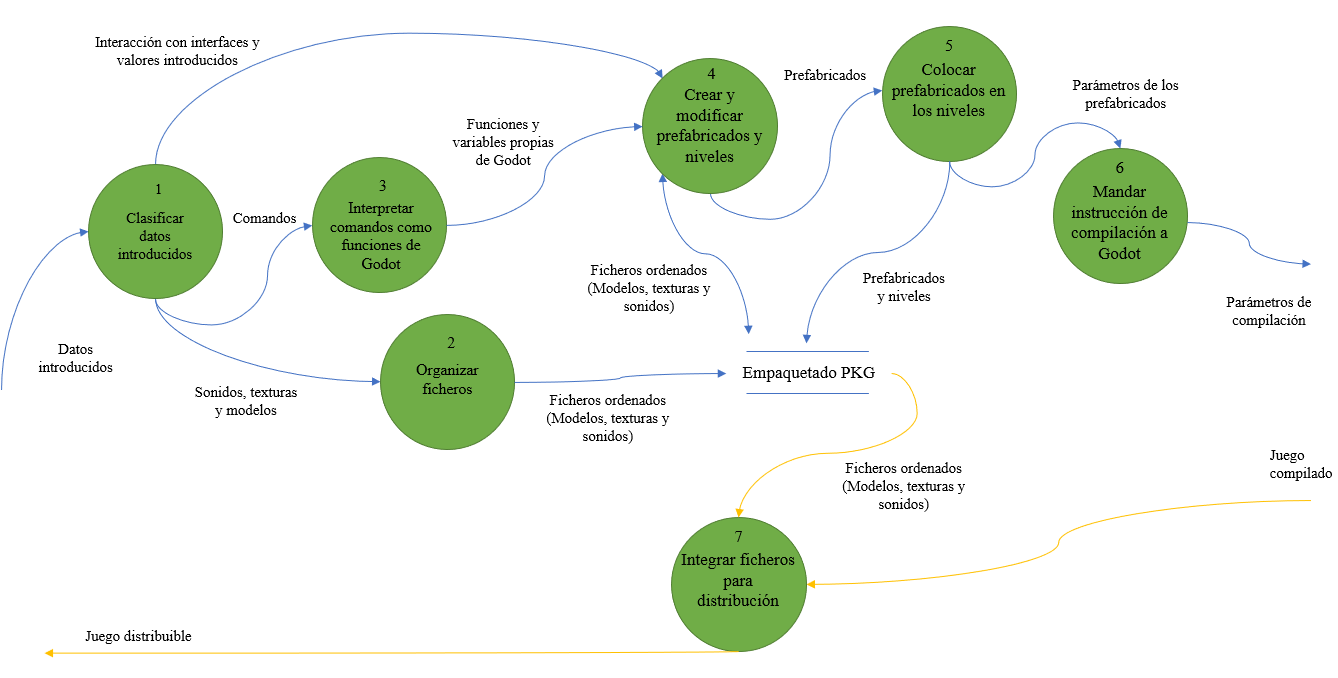
\includegraphics[width=1\textwidth]{DFD2}
	\caption{Diagrama de Flujo de Datos, Nivel 1.} 
	\label{DFD1}
	
\end{figure}




  



\newpage
\part{Entregable 2}
\section{Norma Mexicana}
\subsection{Generalidades}
Framework para crear juegos 3d cuya mec\'anica principal sean los disparos, orientado al rango desde desarrolladores reci\'en iniciados o por iniciarse en el \'ambito, hasta aquellos con conocimiento avanzado. Se compone de una serie de editores entre los cuales se encuentran:
\begin{itemize}
	\item Personajes: Usando una interf\'az simple que permita unificar Inteligencia Artificial, Modelos, animaciones y sonidos. 
	\item Inteligencia Artificial: Mediante un \'arbol de comportamiento.
	\item Niveles: Interf\'az que permita dise\~nar niveles estilo BSP utilizando CSG, evitando as\'i los inconvenientes del alg\'oritmo BSP, pero manteniendo la facilidad de dise\~no que provee. 
	\item Scripts: Mediante un editor ASCII o visual, a elecci\'on del usuario, con la posibilidad de combinar ambos tipos de scripts. 
	
\end{itemize}
\subsection{Responsabilidades}
Como administrador del proyecto, se considera a Yael Atletl Bueno Rojas, como l\'ider de programaci\'on se considera a Kevin Pe\~a, quien queda a cargo de Jos\'e Vald\'ez.
\subsection{Justificaci\'on del proyecto}
Con el prop\'osito de acelerar el desarrollo de videojuegos al permitir a los desarrolladores enfocarse en los elementos que vuelven \'unicos a sus
juegos en vez de gastar tiempo en componentes b\'asicos comunes en la industria, adem\'as de facilitar el inicio del desarrollo y aprendizaje para aquellos con nulo conocimiento sobre el tema, ya que le permite crear videojuegos sin temor a encontrarse barreras de c\'odigo a todo aquel que lo desee, acrecentando de esta forma la innovaci\'on creativa en la industria.

Al cumplir la doble funci\'on de ser un software R.A.D. (Rapid Application Development) y un Framework, cubre dos campos interrelacionados de la industria que han sido descuidados a trav\'es del tiempo, en cuanto a Shooters respecta. 
Software que funciona con los mismos principios ha quedado obsoleto y olvidado, dejando un hueco que el software existente no podr\'ia llenar debido a su nivel de complejidad.

\subsection{An\'alisis de factibilidad}
\subsubsection{Resumen del an\'alisis}
El proyecto consiste en la creaci\'on de un conjunto de herramientas destinadas a facilitar la creaci\'on de videojuegos, proporcionando una interfaz gr\'afica intuitiva y un lenguaje de programaci\'on de muy alto nivel, perfecto para principiantes.
Propiciar\'a la creaci\'on de videojuegos y ofrecer\'a una introducci\'on din\'amica a la programaci\'on.
\subsubsection{Antecedentes}
El proyecto est\'a basado en los trabajos de FPSCreator y Entidad 3d, que permitieron crear juegos de forma r\'apida y sencilla.
Este tipo de herramientas ha demostrado ser adaptado r\'apidamente en las comunidades de creaci\'on de videojuegos. La tecnolog\'ia actual permite la creaci\'on del conjunto de herramientas y su f\'acil mantenimiento.
El funcionamiento de las herramientas se basa en las publicaciones de la Game Development Conference y las publicaciones de Bungie LLC.
\subsubsection{An\'alis del entorno}
\paragraph{Mercado}
Los resultados del ana\'alisis de mercado han dejado en claro los porcentajes de ganancias obtenidos. 

Los Shooters acaparar\'an m\'as de 25.9\% del  mercado americano de los v\'ideo juegos para el a\~no 2019, seg\'un la proyecci\'on basada en la figura~\ref{fig:FORB}  y la figura~\ref{STAT} de la p\'agina~\pageref{STAT}.


\begin{figure}[H]
	
	\centering
	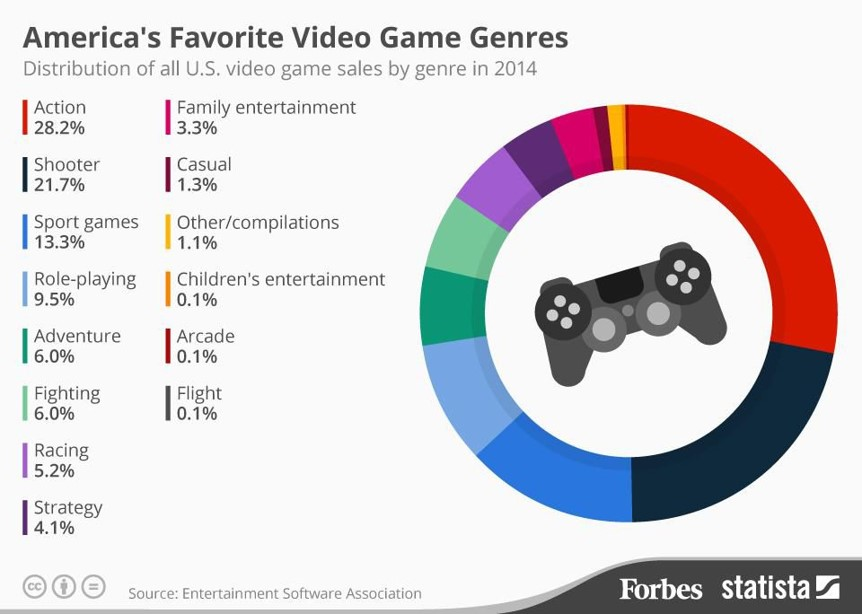
\includegraphics[width=0.5\textwidth]{Picture1}
	\caption{Cuota de mercado, por g\'enero, porcentajes del a\~no 2014.} 
	\label{FORB}
	\cite{Forbes}
	
	
\end{figure}

\begin{figure}[H]
	
	\centering
	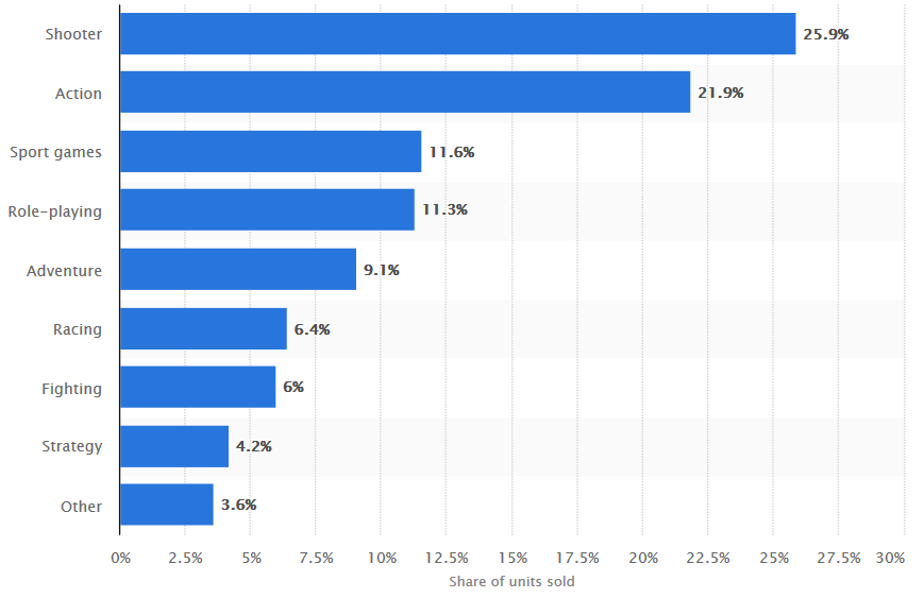
\includegraphics[width=0.5\textwidth]{statista-2}
	\caption{Cuota de mercado, por g\'enero, porcentajes del a\~no 2017.  } 
	\label{STAT}
	\cite{Statista}
	
	
\end{figure}

Estados Unidos es el segundo mayor cosumidor a nivel global, con ingresos de \$32.7 mil millones de d\'olares, tan solo \$7.5 mil millones debajo de China, tal como puede verse en la figura \ref{ENWZOO}.
El motivo para elegir al mercado am\'ericano sobre al chino, es la libertad de publicaci\'on y contenido que existe en \'este; a diferencia de China, donde los videojuegos est\'an regulados por fuertes restricciones y filtros impuestos por el gobierno. \cite{china1}.
%Añadir bibliografía

\begin{figure}[H]
	
	\centering
	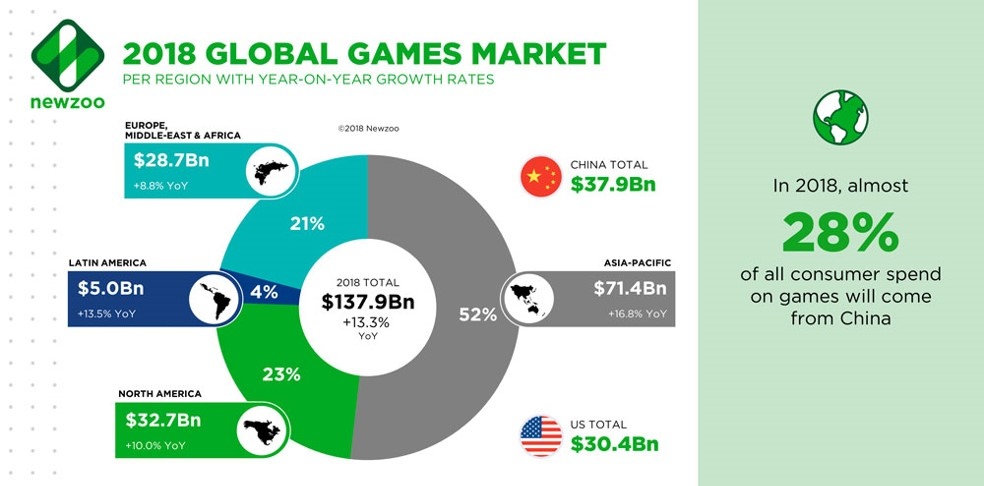
\includegraphics[width=1\textwidth]{GGM2}
	\caption{Procedencia de los ingresos anuales, 2018.  } \cite{Newzoo} 
	\label{ENWZOO}
	
\end{figure}

Considerando los puntos anteriores, es posible calcular una estimaci\'on de ingresos para los shooters en el a\~no 2019:
Con un 1.4\% de crecimiento anual para shooters, lo cual le dejar\'ia un 28.7\% del mercado, que lograr\'a ingresos de 155.827 mil millones de d\'olares, considerando que 35.97 MMDD provendr\'an de Am\'erica del Norte se estiman m\'as de 10.32 MMDD de d\'olares en ganancias para shooters en este 2019. 
\paragraph{Competencia}
A pesar de que la competencia directa es casi inexistente, est\'an presentes otros tipos de competencia, como la competencia de los motores base. Consid\'erese que la tecnolog\'ia base de este proyecto es Godot Engine.

Por un lado es importante destacar que Godot Engine es el motor con mejor percecpi\'on entre sus usuarios, es decir, quienes lo usan est\'an muy satisfechos con las prestaciones del mismo, esto puede notarse en la figura \ref{SLANT}.
 
\begin{figure}[H]
	
	\centering
	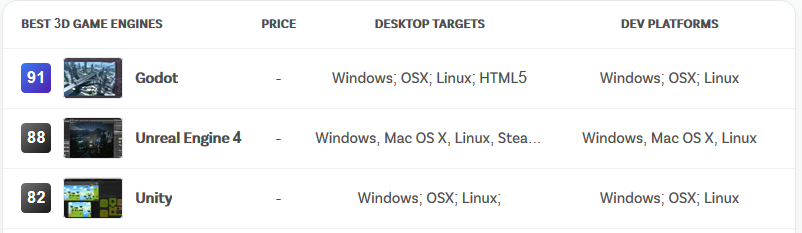
\includegraphics[width=1\textwidth]{Ranking}
	\caption{Ranking de opini\'on de usuarios.  } \cite{Slant} 
	\label{SLANT}
	
\end{figure}

Sin embargo, el motor m\'as utilizado a nivel global es Unity, el cual tiene una gran cantidad de usuarios y una tasa de crecimiento considerable, podemos ver un aumento de m\'as de mil usuarios entre 2018 y 2019, como se nota en las figuras \ref{GGJ2018} y  \ref{GGJ2019}. Consid\'ere a los usuarios como clientes potenciales. Esta es una diferencia que buscamos sobrepasar, ya que la percepci\'on de Unity ante sus usuarios no es excelente, adem\'as de haber alejado a varios desarrolladores desp\'ues de un conflicto de inter\'es con Improbable \cite{Improbable}. 

\begin{figure}[H]
	
	\centering
	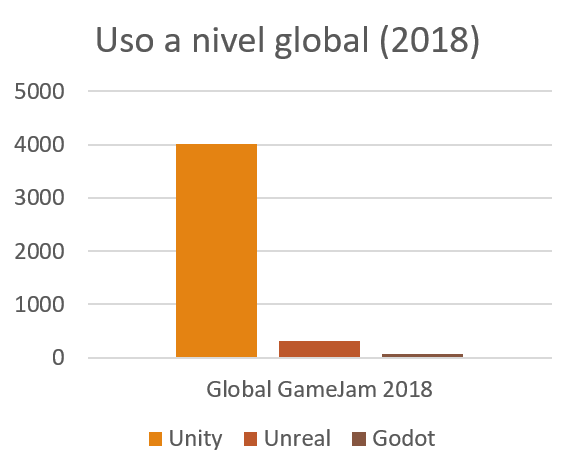
\includegraphics[width=0.5\textwidth]{GGJ}
	\caption{Juegos creados en el Global Game Jam 2018} \cite{GGJ2018} 
	\label{GGJ2018}
	
\end{figure}

\begin{figure}[H]
	
	\centering
	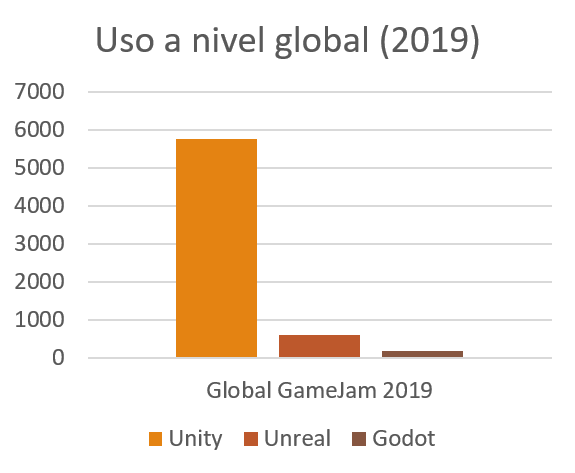
\includegraphics[width=0.5\textwidth]{GGJ2019}
	\caption{Juegos creados en el Global Game Jam 2019} \cite{GGJ2019} 
	\label{GGJ2019}
	
\end{figure}

\subsubsection{Estudio del estado de la t\'ecnica}

\paragraph{Patentes concedidas}
\begin{itemize}
	\item Game production tool supporting multi platform using game development tool. \cite{multip}
	\item Visual game level editing method and system based on trigger. \cite{leveledit}
	\item Server synchronization graph handle tools. \cite{Server}
	\item Tool for video game application development. \cite{EA}
	\item Educational game engine capable of directly developing and combining content. \cite{Edu}
\end{itemize}


\paragraph{Art\'iculos y publicaciones}
Respecto al funcionamiento e implementaci\'on de la tecnolog\'ia, nos hemos basado en diferentes publicaciones: 
\begin{itemize}
	\item ''Evolving Halo's Behaviour Tree AI'' por Max Dyckhoff, para el editor de comportamientos de la IA. \cite{Bungie}
	\item ''What do game developers expect from development and design tools?'' por Jussi Kasurinen, Jukka-Pekka Strand\'en y Kari Smolander, para la flexibilidad y el flujo de trabajo. \cite{ACM}
\end{itemize}
\paragraph{Tecnolog\'ias Disponibles}
La tecnolog\'ia disponible podr\'ia ser clasificada en tecnolog\'ias en bruto y compuestas. En las tecnolog\'ias en bruto est\'an aquellas que no han sido implementadas, es decir, son bibliotecas y APIs de desarrollo: 
\begin{itemize}
	\item OpenGL
	\item Vulkan
	\item DirectX
	\item OpenXR
	\item MotionLeap
	\item OculusVR
	\item SteamVR
	\item SimplexNoise
\end{itemize}
En las tecnolog\'ias compuestas se encuentran los motores de videojuegos, los cuales impementan las tecnolog\'ias en bruto y proveen una integraci\'on \'util.
Como por ejemplo: 
\begin{itemize}
	\item Unity
	\item Unreal Engine 4
	\item Godot Engine
	\item Panda3d
	\item Xenko
	\item Armory3D
	\item CryEngine
	\item Lumberyard
\end{itemize}

\paragraph{Productos en el mercado}
Los productos en el mercado que compiten directamente con el Framework son: 
\begin{itemize}
	\item Entidad 3d
	\item GameGuru
	\item Silentwalk FPS 
	\item FPS Creator
	\item Reality Factory
	
\end{itemize}
Sin embargo, estos est\'an desactualizados o abandonados, con excepci\'on de GameGuru, que est\'a gr\'aficamente rezagado pero es vigente en el mercado. 

\subsubsection{Programa general de trabajo}

El trabajo se ha dividido en dos entregables, la documentaci\'on y las herramientas. De parte de la documentaci\'on, se redactar\'an tutoriales y ejemplos, que ser\'an alojados en un sitio web. \newline
En el caso de las herramientas, se dividen en tres componentes b\'asicos, la interfaz para comunicar al usuario con el motor, los prefabricados que conformar\'an la base del juego y las bibliotecas que permiten el funcionamiento de los prefabricados y la interfaz. V\'ease la figura~\ref{EDT2}

\begin{figure}[H]
	
	\centering
	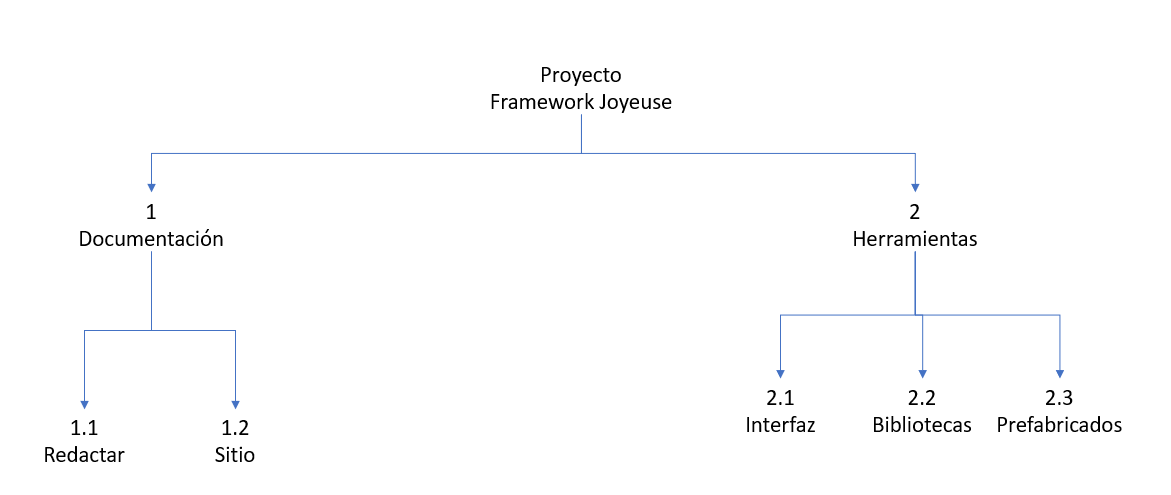
\includegraphics[width=1\textwidth]{EDT}
	\caption{Estructura de desglose de trabajo.} 
	\label{EDT2}
	
\end{figure}
\subsubsection{Determinaci\'on de recursos}
Como recursos humanos se consideraran a Kevin Pe\~a Mora, Jos\'e Vald\'ez y Yael Atletl. En el aspecto financiero, se aproximan \$500 por turno para cada desarrollador, m\'as \$250 por consumo el\'ectrico mensual. 
Para el \'ambito t\'ecnico se utilizar\'an Godot, Github, Sphinx, TravisCI y Read The Docs.

\subsubsection{Aportaci\'on del proyecto}
En el aspecto social/acad\'emico, se busca proporcionar un medio din\'amico para la ense\~nanza de la programaci\'on, accesible para cualquiera. 

Mientras que por el acercamiento econ\'omico permite la creaci\'on de contenido en poco tiempo, minimizando los gastos de producci\'on y permitiendo el lanzamiento temprano. Tambi\'en mejora los tiempos de depuraci\'on y correcci\'on de errores. 

Como impacto secundario al econ\'onmico, para el cual se posee un amplio repertorio de posibilidades, la educaci\'on recibir\'ia un apoyo sustancial, ya que se conseguir\'ia acercar a la programaci\'on a cualquier persona con acceso a una computadora. Por otro lado cabe destacar que se lograr\'ia revivir un sector de la industria cuya oferta decay\'o en a\~nos recientes y que a\'un tiene demanda. Dar una herramienta de este tipo para su uso libre, sin l\'imites para el usuario, ya sean estos de tipo comercial, legal o estructural, permitir\'a el nacimiento de juegos m\'as diversos, ya que se borrar\'a la barrera entre desarrolladores, artistas y jugadores.

\subsection{Desarrollo del proyecto} %
\subsubsection{Generalidades}
Una versi\'on m\'as detallada del EDT explica el plan detallado para el desarrollo del proyecto, para alcanzar la estabilidad de los entregables. V\'ease figura \ref{EDT3}.
\begin{figure}[H]
	
	\centering
	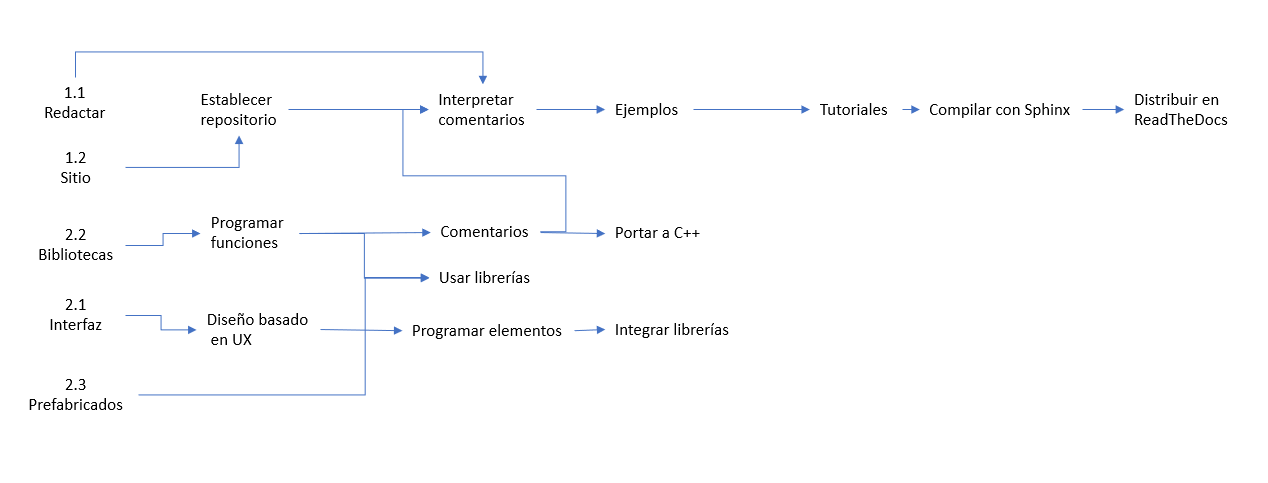
\includegraphics[width=1\textwidth]{EDT2}
	\caption{Estructura de desglose de trabajo detallada.} 
	\label{EDT3}
	
\end{figure} 
\subsubsection{Planificaci\'on de la secuencia}
Se provee en la figura \ref{secuencia} una secuencia detallada de las tareas que ser\'an realizadas, v\'ease el punto ''Interrelaci\'on de tareas'' para m\'as detalles.
\begin{figure}[H]
	
	\centering
	\includegraphics[width=1\textwidth]{secuencia}
	\caption{Secuencia de actividades.} 
	\label{secuencia}
	
\end{figure} 
\subsubsection{Estructura organizativa y personal participante}
Se muestra en la figura \ref{estructura} la jerarqu\'ia organizacional.
\begin{figure}[H]
	
	\centering
	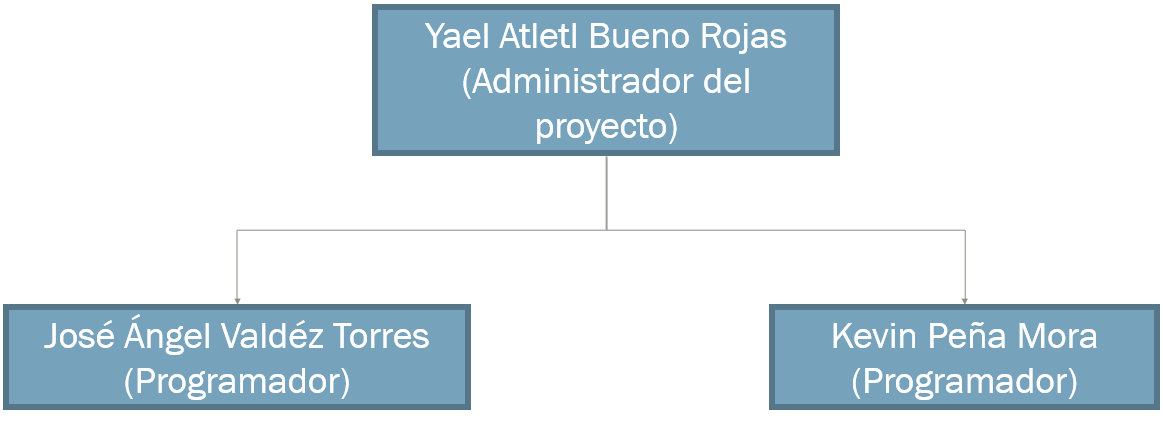
\includegraphics[width=1\textwidth]{estructura}
	\caption{Jerarqu\'ia} 
	\label{estructura}
	
\end{figure} 
\subsubsection{Interrelaci\'on de tareas}
En la figura \ref{rel} se muestra a detalle las tareas que deber\'an realizarse, a la vez que se muestra la secuencia que seguir\'an. 
\begin{figure}[H]
	
	\centering
	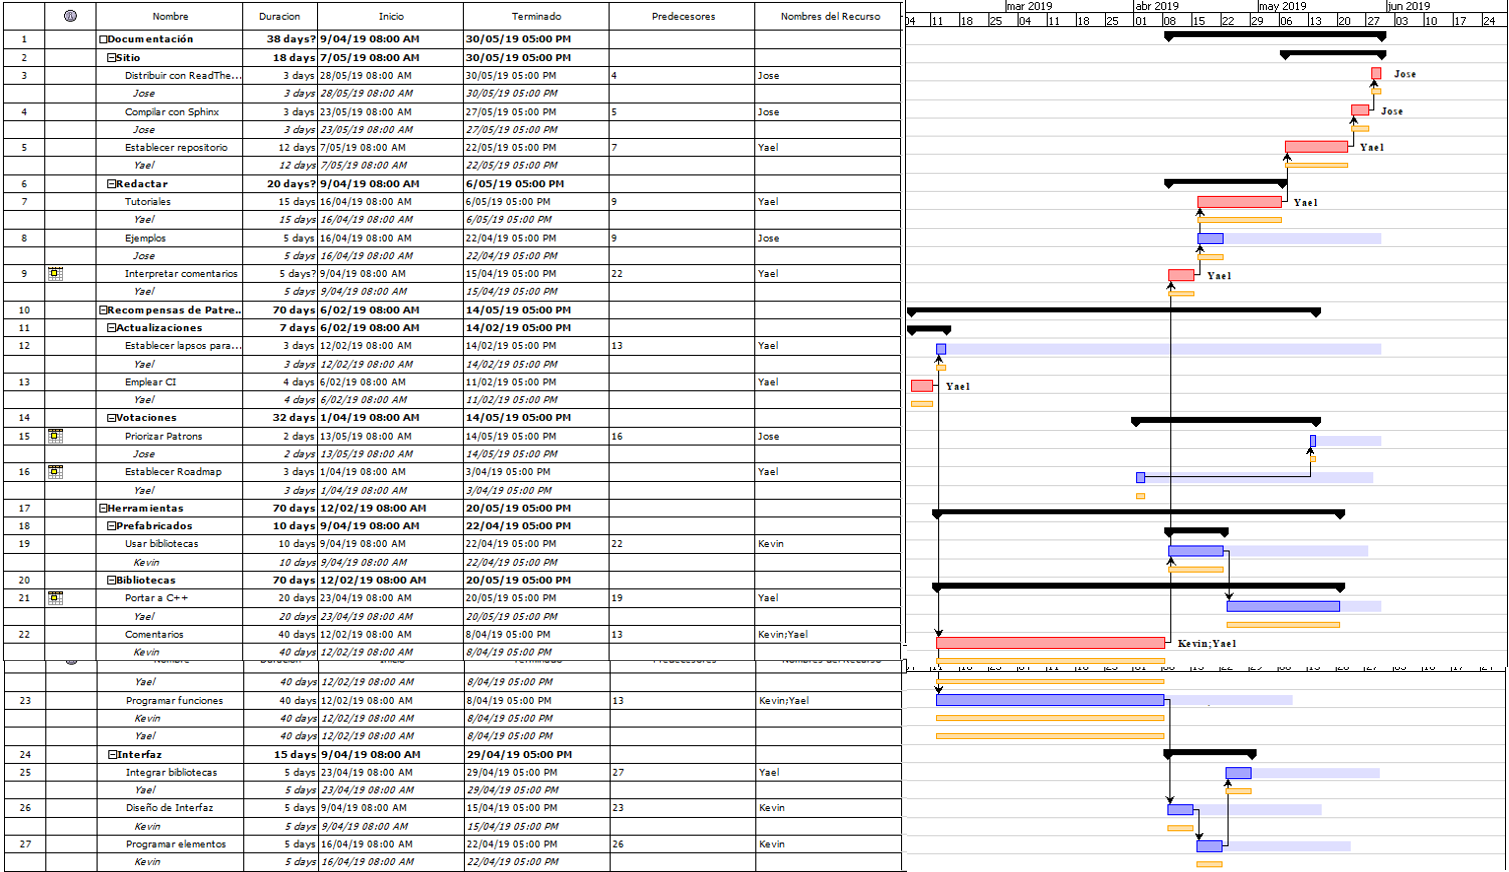
\includegraphics[width=1\textwidth]{relacion}
	\caption{Relaci\'on y secuencia de tareas.} 
	\label{rel}
	
\end{figure} 
\subsection{Presupuesto}
\subsubsection{Recursos asignados}
Como recursos humanos se consideraran a Kevin Pe\~na Mora, Jos\'e Vald\'ez y Yael Atletl. En el aspecto financiero, se aproximan 
Para el \'ambito t\'ecnico se utilizar\'an Godot, Github, Sphinx, TravisCI y Read The Docs.

\subsubsection{Desglose de costos}
\$500 por turno para cada desarrollador, m\'as \$250 por consumo el\'ectrico mensual. 
Considerar el sueldo para el periodo del proyecto para una cuarta persona en caso de ser necesaria la intervenci\'on de un experto para solucionar alg\'un imprevisto que quede fuera del alcance de los integrantes del equipo.

\subsection{Control de programa de proyecto} %
\subsubsection{Identificaci\'on de riesgos}
Se identificaron y categorizaron varios riesgos, mostrados en la figura \ref{ries}.
\begin{figure} [H]
	\centering
	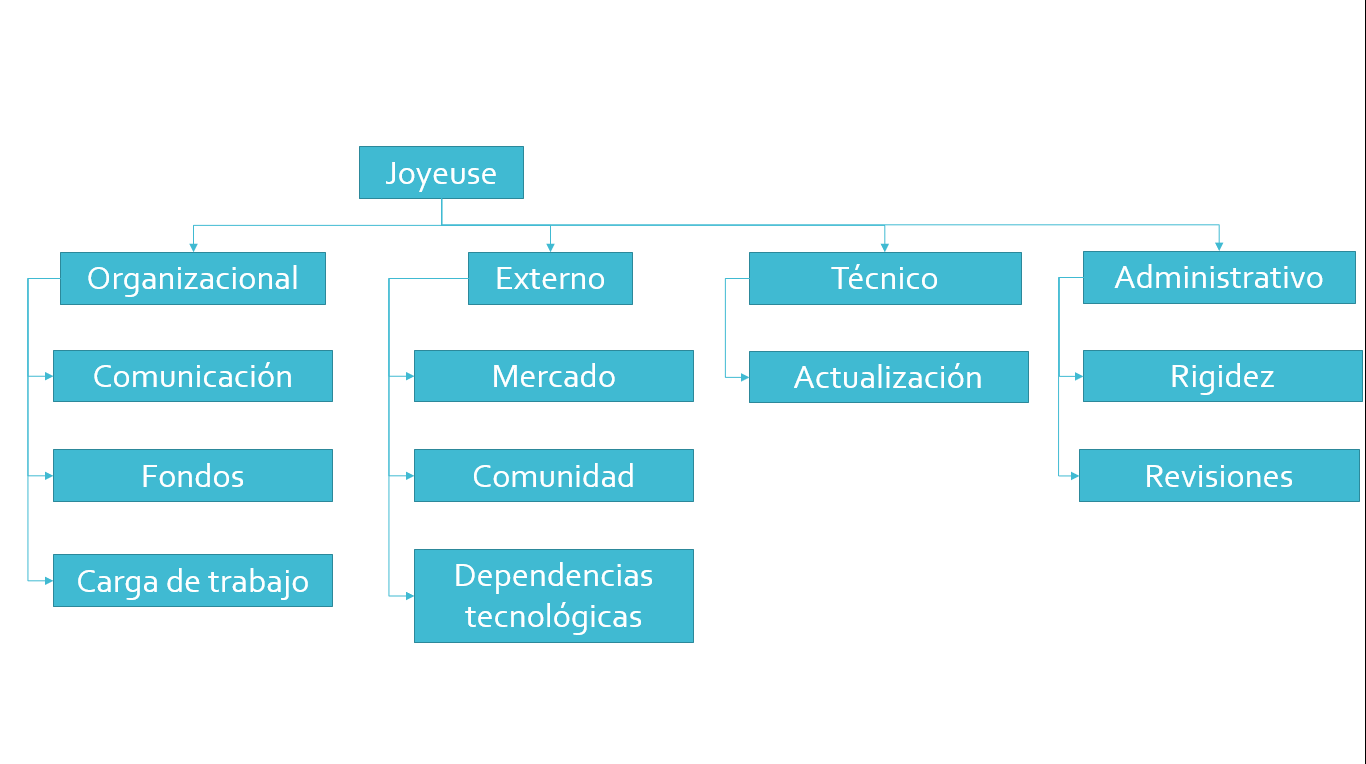
\includegraphics[width=1\textwidth]{RBS}
	\caption{Catergor\'ias de riesgos.} 
	\label{ries}
\end{figure}
Se expande en la identificaci\'on de riesgos, utilizando un diagrama tipo espina de pescado, tal como en la figura \ref{pescado}; de esta forma se facilita la identificaci\'on y la soluci\'on o prevenci\'on de estos. 
\begin{figure} [H]
	\centering
	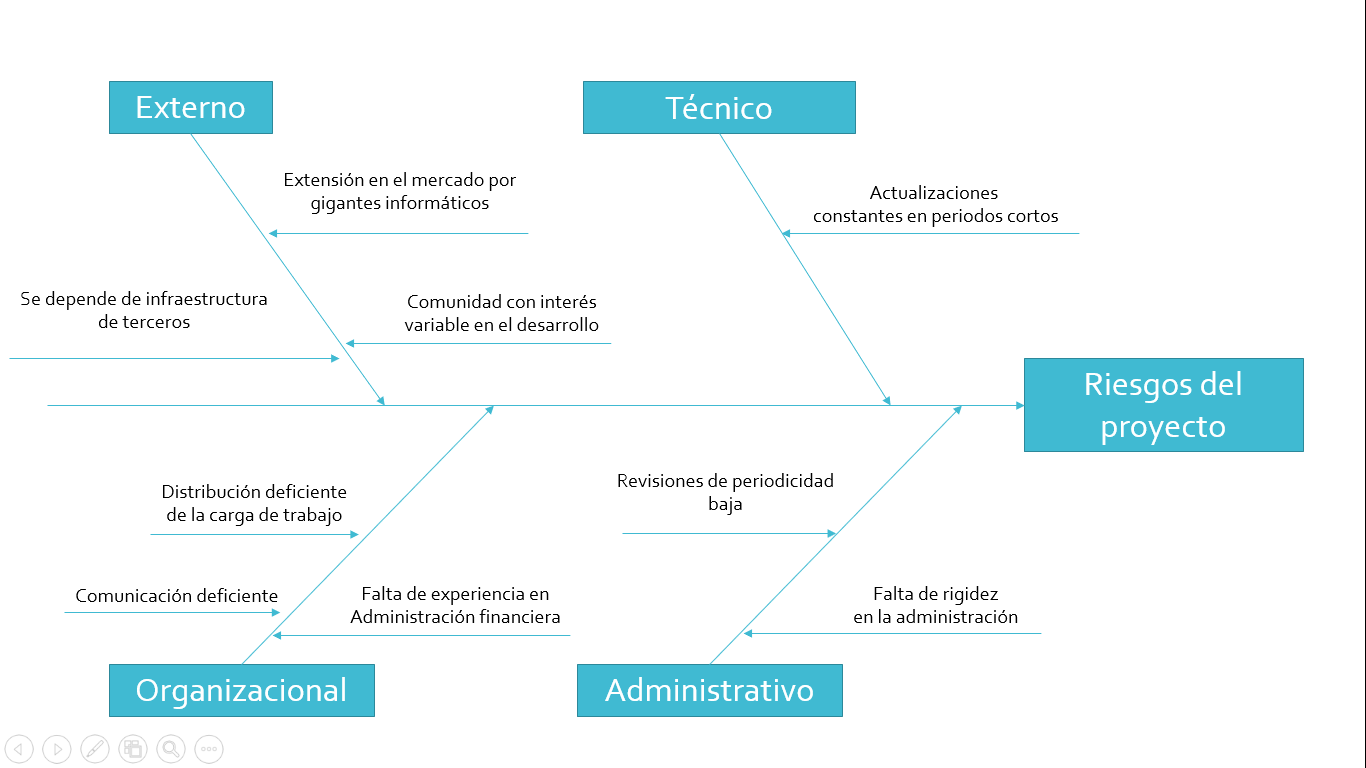
\includegraphics[width=1\textwidth]{Espina}
	\caption{Catergor\'ias de riesgos, con riesgos detallados.} 
	\label{pescado}
\end{figure}

En caso de que los riesgos se presenten y se necesite aplicar una estrat\'egia de soluci\'on, se consiederar\'a un cambio en las estrat\'egias de prevenci\'on, ya que \'estas habr\'an probado ser insuficientes. 

\subsubsection{Gesti\'on de cambios}
Mediante reuniones semanales se identifican los cambios necesarios para el desarrollo del proyecto, basados en los avances actuales y los riesgos que se puedan presentar. Es importante ponderar la posibilidad de que uno de estos riesgos y su impacto en el desarrollo, para de esta forma priorizar aquellos con mayor impacto en el proyecto, en funci\'on de su probabilidad de suceder.
Los cambios y observaciones se registran en las minutas de cada reuni\'on.   

\subsubsection{Medici\'on de avances}

La documentaci\'on del proyecto se divir\'a en 3 entregables, cada uno desde una perspectiva diferente, a medida que se realizan las las actividades de desarrollo como tal, registradas en un log de github y medidas a trav\'es de Milestones (Hitos), que determinar\'an el avance real del proyecto, cada Milestone est\'a contemplado para mes y medio o dos meses de desarrollo, que se alcance o no uno de estos, indicar\'a las estrategias, personal y medidas de prevenci\'on que deber\'an cambiarse o mantenerse. 



\subsection{Protecci\'on del proyecto}
Para la protecci\'on del proyecto se busca establecer una patente y licenciar el contenido bajo una versi\'on modificada de la LGPLv3. Una versi\'on legible para humanos de las condiciones de la licencia ser\'ia la siguiente: 
\newline

Usted puede:
\begin{itemize}
	\item Redistribuir copias f\'isicas de forma comercial o no comercial de los binarios ofrecidos sin modificar. 
	\item Modificar el c\'odigo fuente del framework.
	\item Redistribuir y licenciar el juego producido, sin distribuir el c\'odigo fuente de este. 
\end{itemize}

Usted debe:
\begin{itemize}
	\item Mencionar el uso del Framework en un lugar f\'acilmente visible, como el comienzo de los cr\'editos o la pantalla de inicio del juego. 
	\item Indicar si el Framework ha sido modificado.
	\item Hacer accesible el c\'odigo fuente de cualquier modificaci\'on al Framework. 
\end{itemize}

Usted no deber\'a:
\begin{itemize}
	\item Vender los binarios sin modificar por s\'i solos o como parte de una compilaci\'on, a menos de que sea una distribuci\'on f\'isica.  
	\item Incluir el Framework en los juegos que cree con \'el. (En vez de esto, se recomienda incluir un enlace al sitio oficial del Framework)
\end{itemize}
\section{Conclusiones de la encuesta}
Aqu\'i se tienen los resultados generales y las observaciones obtenidas a trav\'es del an\'alisis de la encuesta que puede encontrarse adjunta a este documento. 
\subsection{Tiempo de desarrollo}
Los apartados que toman mayor tiempo de desarrollo son los elementos gen\'ericos, los personajes y los efectos, seguidos por los niveles. Se descubri\'o que la organizaci\'on de los archivos no suele ser un problema para los usuarios. 
\subsection{Tipo de juego}
Los resultados apuntan a que el estilo de juego preferido por los desarrolladores es un shooter r\'apido, poco estrat\'egico, en primera o tercera persona y de un s\'olo jugador donde se enfrenten a grandes cantidades de enemigos. 
\subsection{Facilidad de uso}
La preferencia es hacia un sistema visual separado de Godot, contenido en un solo ejecutable, el cual recibir\'ia un uso frecuente de tener un editor de personajes. 
\section{Aplicaci\'on de metodolog\'ias \'agiles}
\subsection{Documentaci\'on}

En este caso se utiliza SCRUM, se documentan semanalmente los progresos en el proyecto y se planea el trabajo de la siguiente semana, utilizando minutas tanto para plantear el progreso del desarrollo como el estado de la documentaci\'on. De esta forma se establecen las tareas de la iteraci\'on,s e revisa el progreso y se discuten los retrasos.

\subsection{Desarrollo}

Se utilizar\'a XP (Extreme Programming). Empleando integraci\'on continua se entregan builds preliminares a los usuarios cada d\'ia y se realizan pruebas unitarias. Esto facilita que con Github se les otorgue a los usuarios la capacidad de reportar errores y solicitar caracter\'isticas (se incluye al cliente en el desarrollo), de esta forma se evitan las regresiones y se asegura una entrega de calidad. Despu\'es de cada cierta cantidad de iteraciones se realiza una entrega estable. 

\newpage
\bibliography{Joyeuse}
\bibliographystyle{APA}



\end{document}